\PassOptionsToPackage{table}{xcolor}
\documentclass[nobib,nofonts]{tufte-handout}

%\geometry{showframe} % display margins for debugging page layout

%%% MF additions
% \usepackage[table]{xcolor}
\usepackage[nographicx, nohyperref, nosubcaption, nogb4e, nobiblatex]{../99-auxiliary-files/00-mypackages}
\usepackage{../99-auxiliary-files/00-mycommands}
\usepackage{../99-auxiliary-files/00-myenvironments}

\usepackage{titlesec}
\usepackage{etoolbox}
\usepackage{tikz-qtree}
\usepackage{subcaption}
\usepackage{CSPstyles}

\usepackage{pgfplots}
% externalize PGF plots
% \usepgfplotslibrary{external}
% \tikzexternalize

% \titleformat{\sectionj}
% {\large\bfshape}{\thesection}{1em}{}

\setcounter{secnumdepth}{5}
\renewcommand\thesection{\arabic{section}}

% this length controls tha hanging indent for titles
% change the value according to your needs
\newlength\titleindent
\setlength\titleindent{0.7cm}

\pretocmd{\paragraph}{\stepcounter{subsection}}{}{}
\pretocmd{\subparagraph}{\stepcounter{subsubsection}}{}{}

\titleformat{\chapter}[block]
  {\normalfont\huge\bfseries}{}{0pt}{\hspace*{-\titleindent}}

\titleformat{\section}
  {\normalfont\Large\itshape}{\llap{\parbox{\titleindent}{\thesection\hfill}}}{0em}{}

\titleformat{\subsection}
  {\normalfont\itshape}{\llap{\parbox{\titleindent}{\thesubsection\hfill}}}{0em}{}

\titleformat{\subsubsection}
  {\normalfont\normalsize\itshape}{\llap{\parbox{\titleindent}{\thesubsubsection}}}{0em}{}

\titleformat{\paragraph}[runin]
  {\normalfont\normalsize\itshape}{}{-0.7cm}{}[\xspace \ \ \ \ ]

\titleformat{\subparagraph}[runin]
  {\normalfont\normalsize}{\llap{\parbox{\titleindent}{\thesubsubsection\hfill}}}{0em}{}

\titlespacing*{\chapter}{0pt}{0pt}{20pt}
\titlespacing*{\subsubsection}{0pt}{3.25ex plus 1ex minus .2ex}{1.5ex plus .2ex}
\titlespacing*{\paragraph}{0pt}{3.25ex plus 1ex minus .2ex}{0em}
\titlespacing*{\subparagraph}{0pt}{3.25ex plus 1ex minus .2ex}{0em}

\DefineNamedColor{named}{mygray2}{cmyk}{0.55,0.25,0.25,0.25}
\newcommand{\mygray}[1]{\textcolor{mygray2}{#1}}

%%% Tufte style
\usepackage{graphicx} % allow embedded images
  \setkeys{Gin}{width=\linewidth,totalheight=\textheight,keepaspectratio}
  \graphicspath{{graphics/}} % set of paths to search for images

\usepackage{fancyvrb} % extended verbatim environments
  \fvset{fontsize=\normalsize}% default font size for fancy-verbatim environments

% Standardize command font styles and environments
\newcommand{\doccmd}[1]{\texttt{\textbackslash#1}}% command name -- adds backslash automatically
\newcommand{\docopt}[1]{\ensuremath{\langle}\textrm{\textit{#1}}\ensuremath{\rangle}}% optional command argument
\newcommand{\docarg}[1]{\textrm{\textit{#1}}}% (required) command argument
\newcommand{\docenv}[1]{\textsf{#1}}% environment name
\newcommand{\docpkg}[1]{\texttt{#1}}% package name
\newcommand{\doccls}[1]{\texttt{#1}}% document class name
\newcommand{\docclsopt}[1]{\texttt{#1}}% document class option name
\newenvironment{docspec}{\begin{quote}\noindent}{\end{quote}}% command specification environment

\newcommand{\proplog}{\acro{PropLog}}
\newcommand{\EFSQ}{\ensuremath{\mathit{EFSQ}}\xspace}

\renewcommand{\markdef}[1]{\emph{#1}}

\usepackage{pdfpages}

%%%%%%%%%%%%%%%%%%%%%%%%%%%%%%%%%%%%%%%%%%%%%%%%%%

% \usepackage[sc,osf]{mathpazo}
% \linespread{1.05}


\title{A primer on information theory \\ \normalsize{(for the subjectively perplexed)}}

\author[M.~Franke]{Michael Franke, University of Tübingen, July 2023}


\date{} % without \date command, current date is supplied

\begin{document}

\maketitle

\begin{abstract}
\noindent
Notions covered: information content / surprisal, entropy (joint, conditional, cross), Kullback-Leibler divergence, mutual information.
\end{abstract}

\noindent
Information-theoretic notions ---like entropy, Kullback-Leibler divergence or mutual information--- have many useful applications in fields like statistics, machine learning or computational linguistics.
These notions are anchored in important mathematical results related to efficient coding of information and communication via noisy channels.
However, in order to understand which notion to use when and why in concrete applications, this theoretical grounding in deep and important, but abstract mathematical theory is not always relevant, sometimes possibly even a distraction.
For the student interested in applications, explanations in terms of ``minimal coding length'' or similar can be needlessly confusing at first.
This primer therefore attempts to give a systematic overview of the most salient notions of information theory in terms of what is arguably the pre-theoretically most intuitive perspective: vocabulary about the subjective beliefs of agents.

\section{A measure of information gained}

The centerpiece of information theory is a numerical measure of the amount of information gained, so-called \emph{information content} or \emph{surprisal}.

\subsection{Motivation}

Suppose that Jones and Smith are uncertain about the weather tomorrow at noon.
There are only three possible states of the weather $X = \set{\text{sunny}, \text{misty}, \text{rainy}}$.
Jones' and Smith's subjective beliefs are given in Table~\ref{tab:beliefs-weather}.

\begin{table}
  \centering
  \begin{tabular}{lccc}
    & sunny & cloudy & rainy \\ \midrule
    Jones' beliefs ($P_{J}$)  & 0.6   & 0.2    & 0.2   \\
    Smith's beliefs ($P_{S}$) & 0.1   & 0.2    & 0.7   \\
  \end{tabular}

  \caption{Subjective beliefs about the weather.}
  \label{tab:beliefs-weather}
\end{table}

The next day, Jones and Smith both observe that it is in fact sunny.
Who learns more? Who is more surprised by this turn of events? ---
Intuitively, Smith learns more from the observation of sunny weather (is more surprised by it) than Jones, because Jones had deemed sunny weather rather likely, while Smith had thought that this event is rather unlikely.

This example demonstrates that a measure of the ``information gained'' from the observation of an event $x \in X$ should be sensitive to a baseline probability distribution $P \in \Delta(X)$ such as an agent's prior expectations.
We therefore aim to define a numerical measure $I_{P}(x)$, which assigns a number representing the information gained by observing $x \in X$, given prior beliefs $P \in \Delta(X)$.

There are three further desiderata on the measure $I_{P}(x)$:
\begin{enumerate}
  \item \textbf{Lower bound.} If an agent is already maximally certain that $x$ would occur, $P(x) = 1$, the agent learns nothing from observing $x$, so that $I_{P}(x)=0$.
  \item \textbf{Monotonicity.} The lower the prior probability of $P(x)$ the more information is gained from (alternatively: the more surprised the agent is by) observing an event $x \in X$.
  \item \textbf{Additivity.} If an agent observes two independent events $x_{1}, x_{2} \in X$, the total information gained should be the sum of the information gained from each individual information: $I_{P}(x_{1} \& x_{2}) = I_{P}(x_{1}) + I_{P}(x_{2})$.
\end{enumerate}

\subsection{Information content (surprisal)}

A family of functions that satisfies these desiderata is that of negative logarithms (up to a scaling factor).
Most frequently, the logarithm to base 2 is used.\sidenote{
  The choice of 2 relates to encoding information in binary code, but that is not necessary for a first understanding of the information theoretic notions introduced here.}


Let $P\in \Delta(X)$ be a probability distribution over (finite) set $X$.\sidenote{
  All definitions in this primer are given only for finite sets.
  Generalizations to infinite sets preserve the main intuitions behind the concepts.
}
For event $x \in X$, the \emph{information content} $I_{P}(x)$ of $x$ (a.k.a.~\emph{surprisal} of $x$) is defined as:
\begin{align*}
  I_{P}(x) = - \log_{2} P(x)
\end{align*}
Intuitively speaking, the information content $I_{P}(x)$ is a measure of how surprised an agent with beliefs $P$ is (alternatively: how much the agent learns) when they observe $x$.
Figure~\ref{fig:log-surprisal} shows the information content $I_{P}(x)$ as a function of $P(x)$.
Notice that an agent who assigns $P(x) = 0$ to some event, and sees $x$ happening, is infinitely perplexed (has their mind blown).

\begin{figure}
  \centering
%   \begin{tikzpicture}
% \begin{axis}[
%     width      = 8cm,
%     height     = 6cm,
%     axis lines = left,
%     xlabel     = \(x\),
%     ylabel     = {\(\log_{2} x\)},
% ]
% %Below the red parabola is defined
% \addplot [
%     domain=-0:4,
%     samples=50,
%     very thick,
%     color=mygray2,
%     ]
%     {log2(x)};

% \addplot[
%     mark=none,
%     dotted,
%     domain=-0:4,
%     black,
%     samples=2,
%     ] {0};

% \end{axis}
% \end{tikzpicture}
% \hfill
\begin{tikzpicture}
\begin{axis}[
    width      = 8cm,
    height     = 6cm,
    axis lines = left,
    xlabel = \(P(x)\),
    ylabel = {\(I_{P}(x)\)},
]
%Below the red parabola is defined
\addplot [
    domain=-0:1,
    samples=50,
    very thick,
    color=mygray2,
    ]
    {-log2(x)};

\addplot[
    mark=none,
    dotted,
    domain=-0:1,
    black,
    samples=2,
    ] {0};

\end{axis}
\end{tikzpicture}

\caption{Information content / surprisal (to base 2) for an event $x$ as a function of its prior probability $P(x)$.}
\label{fig:log-surprisal}
\end{figure}

\subsection{Excursion: Background on logarithms}

The logarithm is the inverse function to exponentiation:
\begin{align*}
   x = b^{y} \ \ \ \  \Leftrightarrow  \ \ \ \  y = \log_{b} x
\end{align*}
Here, $b > 0$ is called the \emph{base} of the logarithm.
Since $b^{y}$ is always positive, the logarithm takes as input only positive numbers.
Figure~\ref{fig:logarithm} shows the logarithm to base 2.

\begin{figure}
  \centering
  \begin{tikzpicture}
\begin{axis}[
    width      = 8cm,
    height     = 6cm,
    axis lines = left,
    xlabel     = \(x\),
    ylabel     = {\(\log_{2} x\)},
]
%Below the red parabola is defined
\addplot [
    domain=-0:4,
    samples=50,
    very thick,
    color=mygray2,
    ]
    {log2(x)};

\addplot[
    mark=none,
    dotted,
    domain=-0:4,
    black,
    samples=2,
    ] {0};

\end{axis}
\end{tikzpicture}

\caption{Logarithm to base 2.}
\label{fig:logarithm}
\end{figure}

For present purposes, the following calculation rules are important:\sidenote{
  The first equation is what justifies using logarithms to fulfill the desideratum ``additivity'' given above.
  The second equation will be used in more compact formulations of Kullback-Leibler divergence and mutual information (see below).}
\begin{align*}
  \log_{b}( x y ) & = \log_{b} x + \log_{b} y \\
  \log_{b} \frac{x}{y} & = \log_{b} x - \log_{b} y
\end{align*}
Notice that we can also transform bases of logarithms as follows:
\begin{align*}
  \log_{a} x = \frac{\log_{b} x}{\log_{b} a}
\end{align*}
Since $\log_{b} a$ is a constant (independent of $x$), the choice of base in the definition of information content is, mathematically speaking, arbitrary.

\section{Measures of expected information content}

The most frequently used measures of information theory fall into one of two categories.
For one there are \emph{measures of expected information content}.
These measures are discussed in this section.
They follow the general format:
\begin{align*}
  \sum_{x \in X} \text{Probability of } x \ \times \text{Info-content of } x
\end{align*}
Different measures of this format differ in what kind of distributions are used to define the probability of $x$ and the information content of $x$.

The other class of information-theoretic measures commonly used in applications are \emph{measures of expected difference in information content}.
These measures are dealt with in Section~\ref{sec:meas-expect-diff}, and they instantiate the template:
\begin{align*}
  \sum_{x \in X} \text{Probability of } x \ \times (\text{ Inf.cont } x \text{ wrt. Q } - \text{ Inf.cont. } x \text{ wrt. P })
\end{align*}
where information content is measured based on two different distributions $P$ and $Q$.

\subsection{Entropy}

Let $P\in \Delta(X)$ be a probability distribution over (finite) set $X$.
The \emph{entropy} $\mathcal{H}(P)$ of $P$ is the expected information content under the assumption that the true distribution is $P$:\sidenote{
  Here and below, writing ``true distribution'' or similar formulations does not necessarily entail a strong commitment to actual truth.
  It is shorthand for more careful but cumbersome language like ``the distribution used as a reference or baseline which we assume to be true or treat as if true in order to calculate an expectation.'' }\sidenote{
  We follow common practice here and assume that $0 \log_{a} 0$ = $0$.
  This is justified because $\lim_{x \rightarrow 0^{+}} x \log_{a} x$ = $0$.
}
\begin{align*}
  \mathcal{H}(P) & = \sum_{x \in X} P(x) \ I_{P}(x) \\
                 & = - \sum_{x \in X} P(x) \ \log_{2} P(x)
\end{align*}
Intuitively speaking, the entropy $\mathcal{H}(P)$ measures the expected (or average) surprisal of an agent whose beliefs are $P$ when the true distribution is $P$.
Entropy can also be interpreted as a measure of uncertainty: the higher the entropy of $P$ the more uncertain an agent with beliefs $P$ is about $X$.


\begin{example}
  The entropy of Jones' beliefs in Table~\ref{tab:beliefs-weather} is:
  \begin{align*}
    \mathcal{H}(P_{J})
 & = - \sum_{x \in \set{\text{sunny}, \text{cloudy}, \text{rainy}}} P_{J}(x) \ \log_{2} P_{J}(x) \\
 & = - (0.6  \log_{2} 0.6
   +  0.2  \log_{2} 0.2
   +  0.2  \log_{2} 0.2) \\
 % & \approx - (0.6 \times -0.74 + 0.4 \times -2.33) \\
 & \approx 1.37
  \end{align*}
  A similar calculation for Smith's beliefs yields: $\mathcal{H}(P_{S}) \approx 1.16$.
  Smith is slightly less uncertain (alternatively: more opinionated) than Jones about the state of the weather.
\end{example}

\subsection{Cross entropy}

Let $P, Q \in \Delta(X)$ be probability distributions over (finite) set $X$.
The \emph{cross entropy} $\mathcal{H}(P,Q)$ of probability distributions $P$ and $Q$ measures the expectation of information content given $Q$ from the point of view of the distribution $P$ (which is assumed to be true):
\begin{align*}
  \mathcal{H}(P,Q) & = \sum_{x \in X} P(x) \ I_{Q}(x) \\
                   & = - \sum_{x \in X} P(x) \ \log_{2} Q(x)
\end{align*}
Intuitively speaking, the cross entropy $\mathcal{H}(P,Q)$ measures the expected (or average) surprisal of an agent whose beliefs are $Q$ when the true distribution is $P$.

\begin{example}
  Suppose that Jones is exactly right.
  The beliefs $P_{J}$ capture the precise probability of the weather in the limit (when not taking the weather conditions on the previous days into account).
  Smith's beliefs are therefore not quite in line with reality.
  The cross entropy $\mathcal{H}(P_{J}, P_{S})$ then measures Smith's average surprisal by taking the real-world frequencies $P_{J}$ to form the expectation and by using Smith's beliefs $P_{S}$ to define the surprisal:
  \begin{align*}
    \mathcal{H}(P_{J}, P_{S}) & = - \sum_{x \in X} P_{J}(x) \ \log_{2} P_{S}(x) \\
    & = -( 0.6 \log_{2} 0.1  +
    0.2 \log_{2} 0.2  +
      0.2 \log_{2} 0.7  ) \\
    & \approx 2.56
  \end{align*}
\end{example}


\subsection{Joint entropy}

Joint entropy is entropy for joint probability distributions.\sidenote{
  Here, we only look at structured spaces with two dimensions. Joint entropy can be generalized to further dimensions in an analogous manner.}
Let $R \in \Delta(X \times Y)$ by a joint probability distribution over the set of all pairs in the structured (finite) event space $X \times Y$, and let $P \in \Delta(X)$ and $Q \in \Delta(Y)$ be the \emph{marginal distributions} over $X$ and $Y$ respectively.\sidenote{
  $P(x) = \sum_{y \in Y} R(x,y)$.
}
The \emph{joint entropy} $\mathcal{H}(P,Q)$ of $P$ and $Q$ is defined as:\sidenote{
  Frequently used definitions of joint entropy use random variables $X$ and $Y$ and read as $\mathcal{H}(X, Y) $ = $ - \sum_{x \in X} \sum_{y\in Y} P(x,y) \log_{2} P(x,y)$, where it is implicitly assumed that there is an encompassing joint probability distribution $P(x,y)$ over pairs of numbers. Giving the definition in the way we do here is more general (beyond random variables), but also makes clear how joint entropy is really nothing special at all, except when you muffle the joint distribution through intransparency with random variable notation.
}
\begin{align*}
  \mathcal{H}(P, Q) & = - \sum_{x \in X} \sum_{y\in Y} R(x,y) \log_{2} R(x,y)
\end{align*}
which is just the entropy of the joint probability distribution $R$:
\begin{align*}
  \mathcal{H}(P, Q) = \mathcal{H}(R) = - \sum_{z \in X \times Y} R(z) \log_{2} R(z)
\end{align*}

\begin{example}

Clark also has beliefs about the weather, but theirs are a joint belief $R \in \Delta(X \times Y)$ about the condition of the weather ($X \in \set{\text{sunny}, \text{cloudy}, \text{rainy}} $) and whether the swallows fly high or low in the evening ($Y \in \set{\text{high}, \text{low}}$), as shown in Table~\ref{tab:joint-prob-Clark}.

  \begin{table}

    \begin{tabular}{lcccr}
           & sunny                 & cloudy                & rainy                 & $\sum$ rows \\ \midrule
      high & $.6 \times .4 = .24$ & $.2 \times .4 = .08$ & $.2 \times .4 = .08$ & .4 \\
      low  & $.1 \times .6 = .06$ & $.2 \times .6 = .12$ & $.7 \times .6 = .42$ & .6 \\ \midrule
      $\sum$ columns & .3 & .2 & .5
    \end{tabular}

  \caption{Clark's joint probabilistic belief about the flying of swallows in the evening and the weather condition the next day.}
  \label{tab:joint-prob-Clark}

\end{table}

\medskip

  The joint entropy of Clark's beliefs can be calculated as:
  \begin{align*}
    \mathcal{H}(R) & = - \sum_{x \in \set{\text{sunny}, \text{cloudy}, \text{rainy}}} \sum_{y \in \set{\text{high}, \text{low}}} R(x,y) \ \log_{2} R(x,y) \\
                   & = - (.24 \log_{2} .24  +
                     .08 \log_{2} .08  +
                     .08 \log_{2} .08  +
                     .06 \log_{2} .06  +
                     \dots
                     ) \\
    & \approx 2.22
  \end{align*}


\end{example}

\subsection{Conditional entropy}

Let $R \in \Delta(X \times Y)$ be a joint probability distribution over the set of all pairs in $X \times Y$, and let $P \in \Delta(X)$ and $Q \in \Delta(Y)$ be the marginal distributions over (finite) $X$ and $Y$ respectively.
The conditional entropy of $P$ given $Q$ is the expected surprisal of observing $x$ after having observed some $y$:
\begin{align*}
  \mathcal{H}(P \mid Q) & = - \sum_{\tuple{x,y} \in X \times Y} R(x,y) \log_{2} R(x \mid y)
                          \\
                        & = - \sum_{\tuple{x,y} \in X \times Y} R(x \mid y) Q(y) \log_{2} R(x \mid y)
                        & \mygray{[\text{Bayes rule}]}
                          \\
                        & = - \sum_{x \in X} \sum_{y \in Y} R(x \mid y) Q(y) \log_{2} R(x \mid y)
                        & \mygray{[\text{split the sum}]}
                          \\
                        & = - \underbrace{\sum_{y \in Y} Q(y)}_{\text{prob.~of $y$}}
                          \underbrace{\sum_{x \in X} R(x \mid y) \log_{2} R(x \mid y)}_{\text{entropy of $R(\cdot \mid y)$}}
                          & \mygray{[Q(y) \text{ ind. of }x]}
\end{align*}
We can also think about conditional entropy as the average uncertainty of an agent about dimension $X$ after observing dimension $Y$.
Indeed, if $P$ and $Q$ are stochastically independent, then $\mathcal{H}(P \mid Q) = \mathcal{H}(P)$:
\begin{align*}
  \mathcal{H}(P \mid Q)
  & = - \sum_{y \in Y} Q(y) \sum_{x \in X} R(x \mid y) \log_{2} R(x \mid y)
  \\
  & = - \sum_{y \in Y} Q(y) \sum_{x \in X} P(x) \log_{2} P(x)
  & \mygray{[\text{stoch. independence}]}
  \\
  & = \sum_{y \in Y} Q(y) \mathcal{H}(P)
  & \mygray{[\text{def. entropy}]}
  \\
  & = \mathcal{H}(P)
  & \mygray{\left[ \sum_{y \in Y} Q(y) = 1 \right]}
\end{align*}


\begin{example}
  Suppose that Clark observes the swallows every night and then makes a weather prediction.
  If $P \in \Delta(X)$ captures Clark's marginal beliefs about the weather and $Q \in \Delta(Y)$ those about the swallows flying, then, from Clark's subjective point of view, the expected surprisal of their weather predictions after having observed the swallows is given by the conditional entropy:
  \begin{align*}
    \mathcal{H}(P \mid Q) & = - \sum_{y \in Y} Q(y)
                          \sum_{x \in X} R(x \mid y) \log_{2} R(x \mid y) \\
                          & = - Q(\text{high}) \ [ R(\text{sunny} \mid \text{high}) \ \log_{2} R(\text{sunny} \mid \text{high})  \\
                          & \ \ \ \ \ \ \ \ \ \ \ \ \ \ \ + R(\text{cloudy} \mid \text{high}) \ \log_{2} R(\text{cloudy} \mid \text{high}) \\
                          & \ \ \ \ \ \ \ \ \ \ \ \ \ \ \ + R(\text{rainy} \mid \text{high}) \ \log_{2} R(\text{rainy } \mid \text{high}) ] + \\
                           &\ \ \  \ \ \ - Q(\text{low}) \ [ R(\text{sunny} \mid \text{low}) \ \log_{2} R(\text{sunny} \mid \text{low})  \\
                          & \ \ \ \ \ \ \ \ \ \ \ \ \ \ \ + R(\text{cloudy} \mid \text{low}) \ \log_{2} R(\text{cloudy} \mid \text{low}) \\
                          & \ \ \ \ \ \ \ \ \ \ \ \ \ \ \ + R(\text{rainy} \mid \text{low}) \ \log_{2} R(\text{rainy } \mid \text{low}) ] \\
                          & = - 0.4 [0.6 \log_{2} 0.6 +  0.2 \log_{2} 0.2 + 0.2 \log_{2} 0.2] + \\
                          & \ \ \ \ - 0.6 [0.1 \log_{2} 0.1 +  0.2 \log_{2} 0.2 + 0.7 \log_{2} 0.7] \\
     & \approx 1.242
  \end{align*}
\end{example}

\section{Measures of expected difference in information content }
\label{sec:meas-expect-diff}

Measures of expected difference in information content essentially compare two probability distributions $P$ and $Q$ following the pattern:
\begin{align*}
  \sum_{x \in X} \text{Probability of } x \ \times (\text{ Inf.cont } x \text{ wrt. Q } - \text{ Inf.cont. } x \text{ wrt. P })
\end{align*}
In general, these measures can be thought of as answers to a question like: ``how much more, on average, would an agent using $Q$ be (needlessly) surprised if the true distribution is $P$?''

\subsection{Kullback-Leibler divergence (relative entropy)}

The \emph{Kullback-Leibler (KL) divergence} (also known as \emph{relative entropy}) measures the expected difference in information content between the distribution $Q \in \Delta(X)$ and the true distribution $P \in \Delta(X)$:
\begin{align*}
  D_{KL}(P \,||\, Q) & = \sum_{x \in X} P(x) \ \left ( I_{Q}(x) - I_{P}(x) \right ) \\
  & = \sum_{x \in X} P(x) \ \log_{2}  \frac{P(x)}{Q(x)}
\end{align*}
Intuitively speaking, the KL-divergence $D_{KL}(P \,||\, Q)$ measures how much more surprised an agent is, on average, when they hold beliefs described by $Q$ instead of the true distribution $P$.

KL-divergence $D_{KL}(P \,||\, Q)$ can be equivalently written in terms of the entropy $\mathcal{H}(P)$ of $P$ and the cross entropy $\mathcal{H}(P,Q)$:\sidenote{
  This reformulation shows that KL-divergence and cross-entropy are exchangeable when the task is to find a distribution $Q$ that approximates a true distribution $P$ (e.g., in machine learning).
  KL-divergence and cross-entropy are exchangeable in such an optimization context since the only difference is a constant additive term $\mathcal{H}(P)$ which does not depend on the to-be-optimized $Q$.
}
\begin{align*}
  D_{KL}(P \,||\, Q) = \mathcal{H}(P,Q) - \mathcal{H}(P)
\end{align*}
% include this as exercise

\begin{example}
  Let's assume, again, that Jones' beliefs $P_{J}$ are the true distribution.
  We want to compute the divergence of Smith's beliefs $P_{S}$ from those of Jones'.
  \begin{align*}
    D_{KL}(P_{J} \,||\, P_{S}) & = \sum_{x \in X} P_{J}(x) \log_{2}  \frac{P_{J}(x)}{P_{S}(x)} \\
                               & = 0.6 \log_{2} \frac{0.6}{0.1} +
                                 0.2 \log_{2} \frac{0.2}{0.2} +
                                 0.2 \log_{2} \frac{0.2}{0.7} \\
    & \approx 1.19
  \end{align*}
  If, reversely, we assume that Smith's beliefs are the ground-truth, and compute the divergence of Jones' beliefs from Smith's, then the result is:
  \begin{align*}
    D_{KL}(P_{S} \,||\, P_{J}) & = \sum_{x \in X} P_{S}(x) \log_{2}  \frac{P_{S}(x)}{P_{J}(x)} \\
                               & = 0.1 \log_{2} \frac{0.1}{0.6} +
                                   0.2 \log_{2} \frac{0.2}{0.2} +
                                   0.7 \log_{2} \frac{0.7}{0.2} \\
    & \approx 1.01
  \end{align*}
  This shows that KL-divergence is not a symmetric measure.\sidenote{
    KL-divergence is therefore not a distance metric (like geometrical distance).
  }
\end{example}


\subsection{Mutual information}

Let $R \in \Delta(X \times Y)$ be a joint probability distribution over the set of all pairs in $X \times Y$, and let $P \in \Delta(X)$ and $Q \in \Delta(Y)$ be the marginal distributions over (finite) $X$ and $Y$ respectively.
The \emph{mutual information} $I(P,Q)$ of $P$ and $Q$ is the expected excess surprisal if the dimensions $X$ and $Y$ are assumed to be stochastically independent:
\begin{align*}
  I(P,Q) & = \sum_{\tuple{x,y} \in X \times Y} R(x,y) \log_{2} \frac{R(x,y)}{P(x) \ Q(y)}
\end{align*}
We can write this more intelligibly in terms of the Kullback-Leibler divergence between true distribution $R$ and the distribution $S \in \Delta(X \times Y)$ which is derived from $P$ and $Q$ by assuming that the dimensions $X$ and $Y$ are stochastically independent, so that $S(x,y) = P(x) \ Q(x)$:
\begin{align*}
  I(P,Q) & =  D_{KL}(R \,||\, S) = \sum_{\tuple{x,y} \in X \times Y} R(x,y) \log_{2} \frac{R(x,y)}{S(x,y)}
\end{align*}
Intuitively, we may think of mutual information as a measure of how much more (needlessly) surprised an agent is who believes $X$ and $Y$ are stochastically independent (while having correct beliefs about the marginal distributions).

Mutual information $I(P,Q)$ can be equivalently expressed in terms of entropy and conditional entropy like so:
\begin{align*}
  I(P,Q) = \mathcal{H}(P) - \mathcal{H}(P \mid Q)
\end{align*}
Based on this reformulation, we can think of mutual information as a measure of the change in uncertainty about $P$ between a state \emph{before} learning about $Q$ and \emph{after} learning about $Q$.
In yet other terms, mutual information captures the reduction of uncertainty about the question ``which $P$?'' after receiving an answer to the question ``which $Q$?''.
If $P$ and $Q$ are stochastically independent, then obtaining an answer to the question ``which $Q$?'' will not tell you anything about the question``which $P$?'', so that in that case $I(P,Q)$ will indeed be zero ($\mathcal{H}(P \mid Q) = \mathcal{H}(P)$ whenever $P$ and $Q$ are independent, as we saw above).


\begin{example}
  Clark has the joint probability distribution $R \in \Delta(X \times Y)$ in Table~\ref{tab:joint-prob-Clark}, whose marginal distributions are $P \in \Delta(X)$ (beliefs about the weather) and $Q \in \Delta(Y)$ (beliefs about the swallows).
  Clark's beliefs are repeated here from above:
  \begin{center}
    \begin{tabular}{lcccr}
                     & sunny & cloudy & rainy & $\sum$ rows \\ \midrule
      high           & $.24$ & $.08$  & $.08$ & .4 \\
      low            & $.06$ & $.12$  & $.42$ & .6 \\ \midrule
      $\sum$ columns & .3    & .2     & .5
    \end{tabular}

  \end{center}
  Jackson has a joint probability distribution $S \in \Delta(X \times Y)$ which assigns the same probabilities to the (marginal) events ``weather condition'' and ``swallows' flying height,'' but which assumes that these dimensions are independent, so that $S(x,y) = P(x) \ Q(y)$.
  This means that Jackson's beliefs are these:
  \begin{center}
    \begin{tabular}{lcccr}
                     & sunny & cloudy & rainy & $\sum$ rows \\ \midrule
      high           & $.12$ & $.08$  & $.20$ & .4 \\
      low            & $.18$ & $.12$  & $.30$ & .6 \\ \midrule
      $\sum$ columns & .3    & .2     & .5
    \end{tabular}
  \end{center}
  If Clark's beliefs are the reference distribution, how much more surprised will Jackson be about the occurrence of pairs $\tuple{x,y}$ on average?
  \begin{align*}
    I(X,Y) & =  D_{KL}(R \,||\, S) = \sum_{\tuple{x,y} \in X \times Y} R(x,y) \log_{2} \frac{R(x,y)}{S(x,y)} \\
           & = R(\text{sunny} , \text{high}) \ \log_{2} \frac{R(\text{sunny} , \text{high})}{Q(\text{sunny} , \text{high})}  \\
           & \ \ \ \ \ \ \ \ \ \ \ + R(\text{cloudy} , \text{high}) \ \log_{2} \frac{R(\text{cloudy} , \text{high})}{Q(\text{cloudy} , \text{high})} \\
           & \ \ \ \ \ \ \ \ \ \ \ + R(\text{rainy} , \text{high}) \ \log_{2} \frac{R(\text{rainy } , \text{high})}{Q(\text{rainy } , \text{high})} \\
           & \ \ \ \ +  R(\text{sunny} , \text{low}) \ \log_{2} \frac{R(\text{sunny} , \text{low})}{Q(\text{sunny} , \text{low})}  \\
           & \ \ \ \ \ \ \ \ \ \ \ + R(\text{cloudy} , \text{low}) \ \log_{2} \frac{R(\text{cloudy} , \text{low})}{Q(\text{cloudy} , \text{low})} \\
           & \ \ \ \ \ \ \ \ \ \ \ + R(\text{rainy} , \text{low}) \ \log_{2} \frac{R(\text{rainy } , \text{low})}{Q(\text{rainy } , \text{low})} \\
    & \approx 0.24
  \end{align*}
\end{example}

\newpage

\bigskip
\noindent \colorbox{mygray}{\centering
  \begin{minipage}{1.0\textwidth}


    \begin{exercise}
      Roberts and Carpenter hold the following beliefs about the weather:

      \begin{center}
        \begin{tabular}{lcccc}
                              & sunny & cloudy & rainy & stormy \\ \midrule
          Roberts' beliefs     & 0.1   & 0.6    & 0.2   & 0.1 \\
          Carpenter's beliefs & 0.4   & 0.1    & 0.3   & 0.2 \\
        \end{tabular}
      \end{center}

        Calculate the entropy of their beliefs. Who is more uncertain?
    \end{exercise}

    \begin{exercise}
      Let the true distribution over weather conditions (ignoring dependencies between consecutive days) be:

      \begin{center}
        \begin{tabular}{lcccc}
                       & sunny & cloudy & rainy & stormy \\ \midrule
          ground truth & 0.7   & 0.1    & 0   & 0.2 \\
        \end{tabular}
      \end{center}

      Calculate the cross-entropy of Robert's and Carpenter's belief with respect to this reference distribution.
      Can you guess who will be more suprised on average?

    \end{exercise}

    \begin{exercise}

      Calculate the KL-divergence between the reference distribution from the previous exercise and Robert's and Carpenter's beliefs (each). (Hint: you might be able to use some results from other exercises.)

    \end{exercise}

    \begin{exercise}
      Proof that indeed, as claimed above, $D_{KL}(P \,||\, Q) = \mathcal{H}(P,Q) - \mathcal{H}(P)$
    \end{exercise}

    \begin{exercise}
      Decide for each of the following claims whether it is true or false?
      \begin{enumerate}[(i)]
        \item Kullback-Leibler divergence is a special case of mutual information.
        \item Kullback-Leibler divergence is a measure of expected information content of the reference distribution.
        \item Joint entropy measures the entropy of joint probability distributions.
        \item Entropy is a measure of the information gained from a single observation.
        \item Mutual information could be used to measure the extent to which making an assumption of stochastic independence is severe.
      \end{enumerate}
    \end{exercise}

  \end{minipage}
}


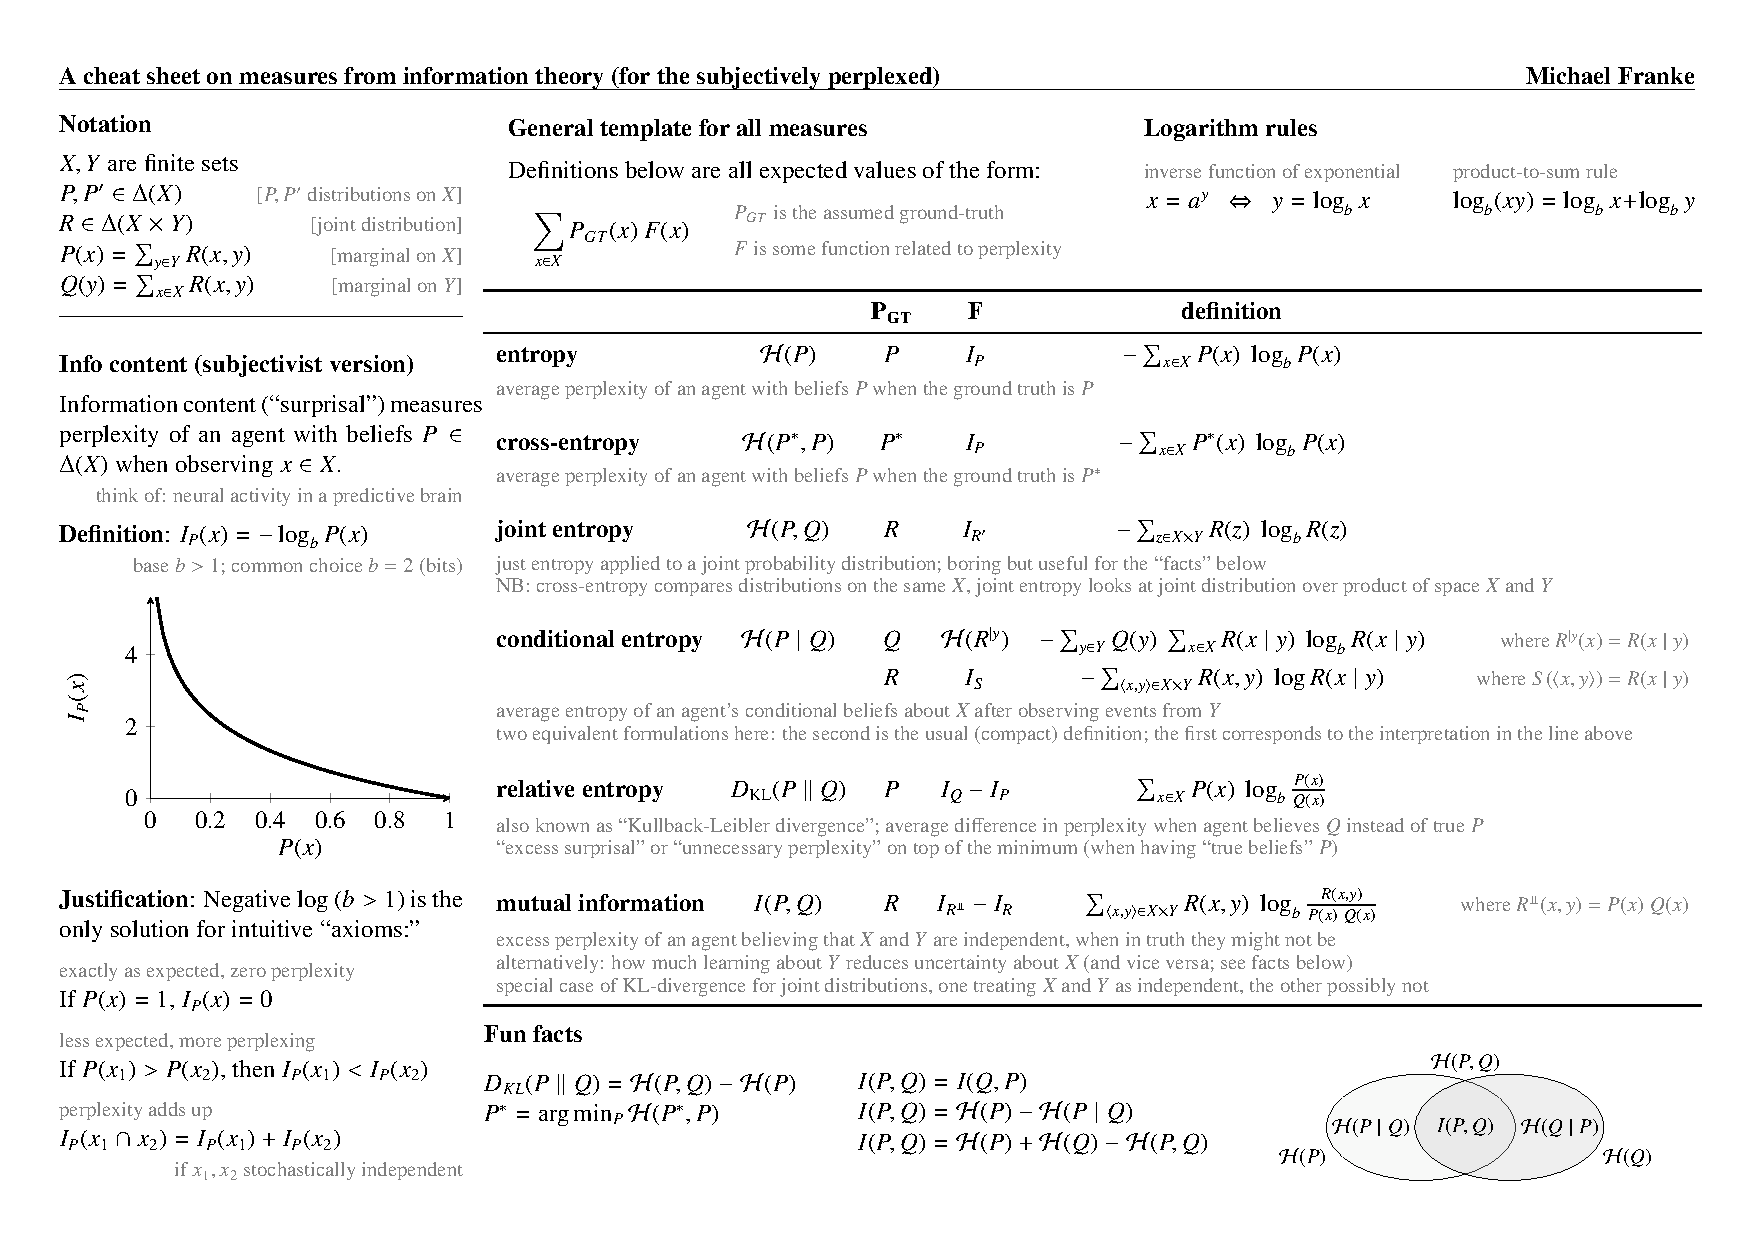
\includepdf[pages={-},fitpaper,rotateoversize]{07-cheat-sheet-info-theory.pdf}


\end{document}

Applications (Gerhard):

entropy as measure of language complexity (e.g., in morphological markers)
mutual information as measure of degree of relatedness between languages
